Identifying hidden communities within networks is a crucial graph analytics problem relevant to various domains, including topic discovery, disease prediction, drug discovery, criminal identification, protein annotation, and inferring land use. The goal is to identify groups of vertices with dense internal connections and sparse connections to the rest of the graph. A challenge in community detection is the absence of prior knowledge about the number and size distribution of communities. To address this, researchers have developed numerous heuristics for finding communities \cite{com-guimera05, com-derenyi05, com-newman06, com-reichardt06, com-raghavan07, com-blondel08, com-rosvall08, infomap-rosvall09, com-fortunato10, com-gregory10, com-kloster14, com-come15, com-ruan15, com-newman16, com-ghoshal19, com-rita20, com-lu20, com-gupta22}. The quality of identified communities is often measured using fitness metrics such as the modularity score proposed by Newman et al. \cite{com-newman06}. These communities are\ignore{considered} intrinsic when identified based solely on network topology\ignore{, without external attributes}, and they are disjoint when each vertex belongs to only one community \cite{com-gregory10}.

The Louvain method, proposed by Blondel et al. \cite{com-blondel08} from the University of Louvain, is one of the most popular community detection algorithms \cite{com-lancichinetti09}. This greedy algorithm employs a two-phase approach, consisting of a local-moving phase and an aggregation phase, to iteratively optimize the modularity metric \cite{com-blondel08}. It has a time complexity of $O(KM)$ (where $M$ is the number of edges in the graph and $K$ is the total number of iterations performed across all passes) and efficiently identifies communities with high modularity.

Despite its popularity, the Louvain method has been observed to produce internally disconnected and poorly connected communities. To address these shortcomings, Traag et al. \cite{com-traag19}, from the University of Leiden, proposed the \textit{Leiden algorithm}. This algorithm introduces an additional refinement phase between the local-moving and aggregation phases. During the refinement phase, vertices can explore and potentially form sub-communities within the communities identified in the local-moving phase. This allows the Leiden algorithm to identify well-connected communities \cite{com-traag19}.\ignore{We have proposed an efficient multicore implementation of Leiden algorithm \cite{sahu2023gveleiden}.}

But many real-world graphs evolve rapidly over time, through the insertion and deletion of edges and vertices. These dynamic graphs are often immense in scale, arising from applications such as machine learning and social networks, and are becoming increasingly ubiquitous. For efficiency, algorithms are needed that update results without recomputing from scratch, known as \textit{dynamic algorithms}. One straightforward strategy for dynamic community detection involves leveraging the community memberships of vertices from the previous snapshot of the graph \cite{com-aynaud10, com-chong13, com-shang14, com-zhuang19}, which we term as \textit{Naive-dynamic (ND)}. Alternatively, more sophisticated techniques have been devised to reduce computational overhead by identifying a smaller subset of the graph affected by changes. These techniques include updating only changed vertices \cite{com-aktunc15, com-yin16}, processing vertices in the proximity of updated edges (within a specified threshold distance) \cite{com-held16}, disbanding affected communities into lower-level networks \cite{com-cordeiro16}, or employing a dynamic modularity metric to recompute community memberships from scratch \cite{com-meng16}. Recently, a technique known as \textit{Delta-screening (DS)} has been proposed, which identifies a subset of vertices impacted by changes in a graph using delta-modularity \cite{com-zarayeneh21}. We have also introduced an efficient incrementally expanding approach for dynamic community detection, which we call the \textit{Dynamic Frontier (DF)} approach \cite{sahu2024dflouvain}.

However, the above\ignore{research} efforts have focused on detecting communities in dynamic networks using the Louvain algorithm. None have extended these approaches to the Leiden algorithm. Further, a majority of the reported algorithms \cite{com-aynaud10, com-chong13, com-meng16, com-cordeiro16, com-zhuang19, com-zarayeneh21} are sequential. Parallel algorithms for graph analytics on dynamic graphs are an active area of research. Examples of parallel dynamic algorithms include those for updating centrality scores \cite{cent-shao20, cent-regunta21}, maintaining shortest paths \cite{path-zhang17, path-khanda21}, and dynamic graph coloring \cite{color-yuan17, color-bhattacharya18}.

This technical report extends the parallel Dynamic Frontier (DF) approach to the Leiden algorithm.\footnote{\url{https://github.com/puzzlef/leiden-communities-openmp-dynamic}} DF Leiden is based on GVE-Leiden \cite{sahu2023gveleiden}, our multicore implementation of the Static Leiden algorithm. Upon receiving a batch update comprising edge deletions and insertions, DF Leiden incrementally identifies and processes an approximate set of affected vertices in an incremental manner. Additionally, we introduce parallel implementations of Naive-dynamic (ND) and Delta-screening (DS) Leiden. This work represents, to the best of our knowledge, the first endeavor in extending existing dynamic approaches to the Leiden algorithm.




%% - Use --- for a dash.
%% - Use ``camera-ready'' for quotes.
%% - Use {\itshape very} or \textit{very} for italicized text.
%% - Use \verb|acmart| or {\verb|acmart|} for mono-spaced text.
%% - Use \url{https://capitalizemytitle.com/} for URLs.
%% - Use {\bfseries Do not modify this document.} for important boldface details.
%% - Use \ref{fig:name} for referencing.

%% For a block of pre-formatted text: 
% \begin{verbatim}
%   \renewcommand{\shortauthors}{McCartney, et al.}
% \end{verbatim}

%% For a list of items:
% \begin{itemize}
% \item the ``ACM Reference Format'' text on the first page.
% \item the ``rights management'' text on the first page.
% \item the conference information in the page header(s).
% \end{itemize}

%% For a table:
% \begin{table}
%   \caption{Frequency of Special Characters}
%   \label{tab:freq}
%   \begin{tabular}{ccl}
%     \toprule
%     Non-English or Math&Frequency&Comments\\
%     \midrule
%     \O & 1 in 1,000& For Swedish names\\
%     $\pi$ & 1 in 5& Common in math\\
%     \$ & 4 in 5 & Used in business\\
%     $\Psi^2_1$ & 1 in 40,000& Unexplained usage\\
%   \bottomrule
% \end{tabular}
% \end{table}

%% For a full-width table:
% \begin{table*}
%   \caption{Some Typical Commands}
%   \label{tab:commands}
%   \begin{tabular}{ccl}
%     \toprule
%     Command &A Number & Comments\\
%     \midrule
%     \texttt{{\char'134}author} & 100& Author \\
%     \texttt{{\char'134}table}& 300 & For tables\\
%     \texttt{{\char'134}table*}& 400& For wider tables\\
%     \bottomrule
%   \end{tabular}
% \end{table*}


%% For inline math:
% \begin{math}
%   \lim_{n\rightarrow \infty}x=0
% \end{math},

%% For a numbered equation:
% \begin{equation}
%   \lim_{n\rightarrow \infty}x=0
% \end{equation}

%% For an unnumbered equation:
% \begin{displaymath}
%   \sum_{i=0}^{\infty} x + 1
% \end{displaymath}

%% For a figure:
% \begin{figure}[h]
%   \centering
%   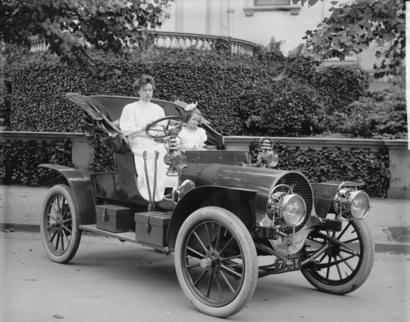
\includegraphics[width=\linewidth]{inc/sample-franklin}
%   \caption{1907 Franklin Model D roadster. Photograph by Harris \&
%     Ewing, Inc. [Public domain], via Wikimedia
%     Commons. (\url{https://goo.gl/VLCRBB}).}
%   \Description{A woman and a girl in white dresses sit in an open car.}
% \end{figure}

%% For a teaser figure.
% \begin{teaserfigure}
%   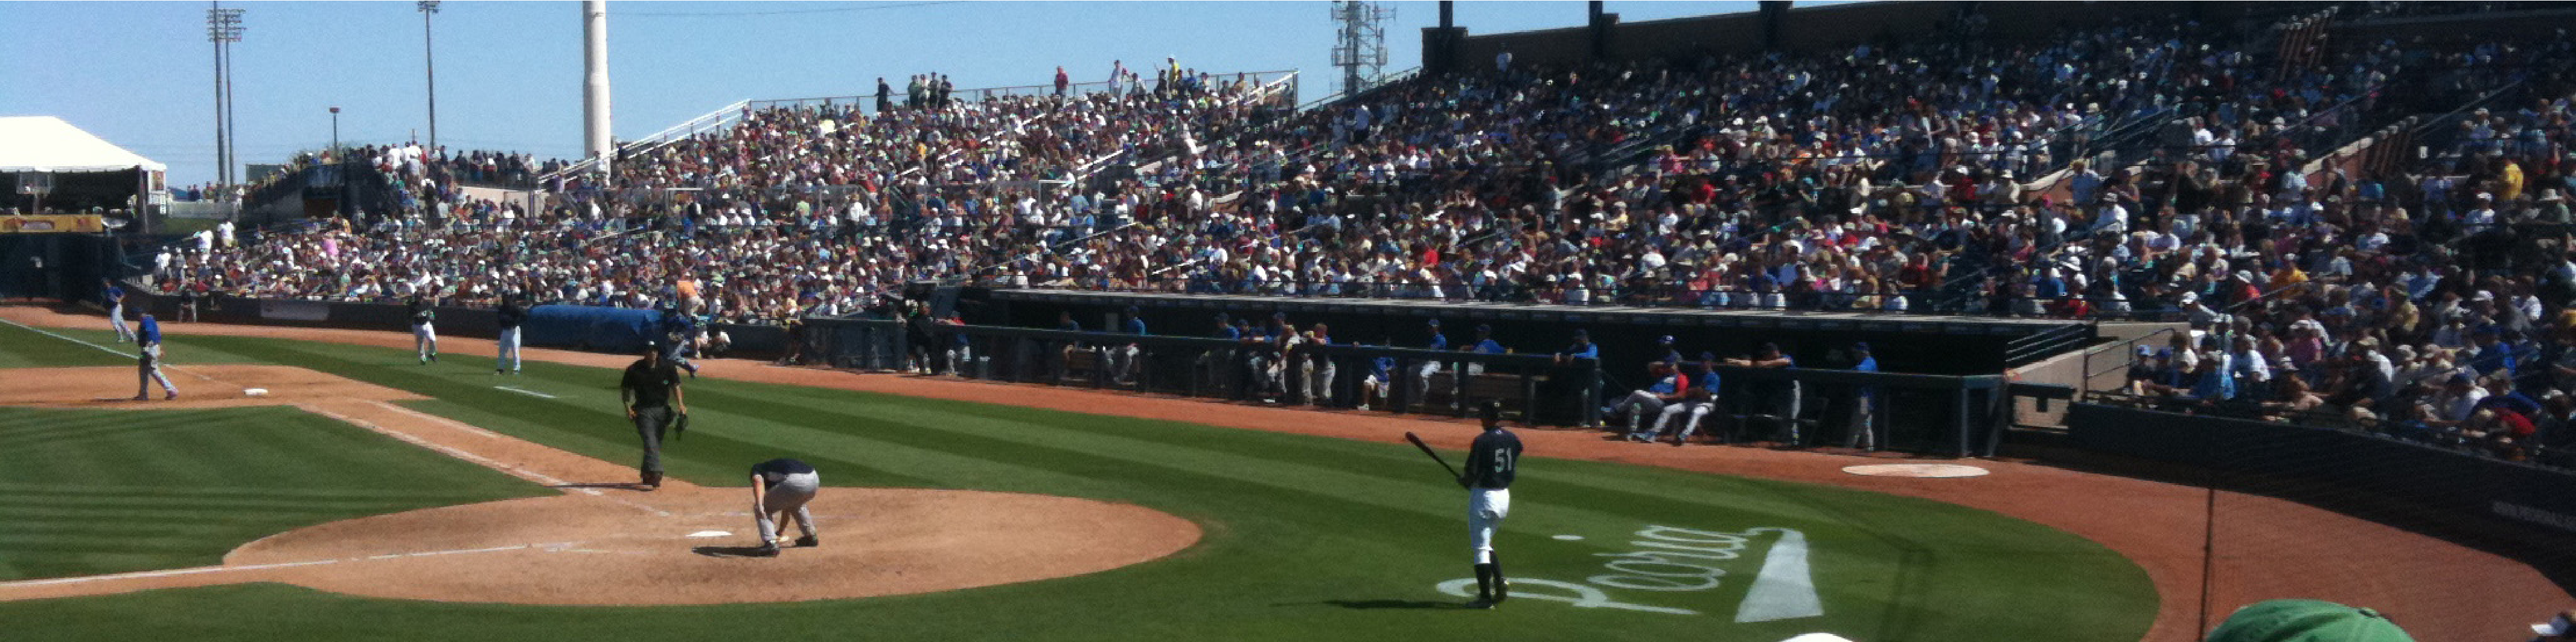
\includegraphics[width=\textwidth]{sampleteaser}
%   \caption{figure caption}
%   \Description{figure description}
% \end{teaserfigure}
